%=========================================================
% Capítulo 3 — Ajuste por mínimos quadrados
%=========================================================
\chapter{Ajuste por mínimos quadrados}
\label{ch:minimos-quadrados}

\noindent\textbf{Resumo:}
Este capítulo introduz o método dos mínimos quadrados como a extensão natural da interpolação quando os dados contêm ruído e inconsistências.  
Mostra-se como o ajuste ótimo busca minimizar o erro global e não o erro pontual, formalizando o conceito de \emph{melhor estimativa}.  
A formulação matricial do problema é apresentada, juntamente com a interpretação geométrica de projeção ortogonal, que mais tarde dará origem à formulação variacional da assimilação de dados.

%---------------------------------------------------------
\section{Motivação: do ajuste exato ao ótimo}
Em situações reais, as observações não são exatas. Cada ponto medido $y_i$ possui um erro associado, e forçar a função a passar exatamente por todos eles pode introduzir oscilações e exagerar o ruído.  
Em vez disso, buscamos uma função $f(x; \mathbf{a})$ parametrizada (por exemplo, um polinômio) que minimize o erro médio ao longo de todos os pontos:
\begin{equation}
J(\mathbf{a}) = \sum_{i=1}^{n} \big[y_i - f(x_i; \mathbf{a})\big]^2.
\label{eq:J_scalar}
\end{equation}
O valor mínimo de $J$ fornece o \emph{melhor ajuste} global — o que explica a sigla \emph{BLUE} (\emph{Best Linear Unbiased Estimator}) que aparecerá mais adiante em AD.

%---------------------------------------------------------
\section{Formulação linear e derivação}
Para um modelo linear nos parâmetros,
\begin{equation}
f(x_i;\mathbf{a}) = \sum_{j=1}^{m} a_j \, \phi_j(x_i),
\label{eq:modelo-linear}
\end{equation}
em que $\phi_j(x)$ são funções base conhecidas (por exemplo, $1$, $x$, $x^2$, ...), podemos reescrever o problema em forma matricial:
\[
\mathbf{y} = \Phi \mathbf{a} + \boldsymbol{\varepsilon},
\]
onde
\[
\Phi =
\begin{bmatrix}
\phi_1(x_1) & \phi_2(x_1) & \dots & \phi_m(x_1) \\
\phi_1(x_2) & \phi_2(x_2) & \dots & \phi_m(x_2) \\
\vdots & \vdots & \ddots & \vdots \\
\phi_1(x_n) & \phi_2(x_n) & \dots & \phi_m(x_n)
\end{bmatrix},
\qquad
\mathbf{y} = 
\begin{bmatrix}
y_1 \\ y_2 \\ \vdots \\ y_n
\end{bmatrix},
\quad
\mathbf{a} = 
\begin{bmatrix}
a_1 \\ a_2 \\ \vdots \\ a_m
\end{bmatrix}.
\]
O vetor de resíduos é $\boldsymbol{r} = \mathbf{y} - \Phi\mathbf{a}$.  
Minimizar $J=\boldsymbol{r}^\top\boldsymbol{r}$ leva à condição normal:
\begin{equation}
\frac{\partial J}{\partial \mathbf{a}} = -2 \Phi^\top (\mathbf{y} - \Phi\mathbf{a}) = 0,
\label{eq:gradJ}
\end{equation}
resultando nas \emph{equações normais}:
\begin{equation}
\Phi^\top \Phi \, \mathbf{a} = \Phi^\top \mathbf{y}.
\label{eq:normal-equations}
\end{equation}
A solução é dada por:
\begin{equation}
\boxed{\mathbf{a} = (\Phi^\top \Phi)^{-1}\Phi^\top \mathbf{y}.}
\label{eq:LS-solution}
\end{equation}
Essa expressão é a base da estimação linear: a mesma estrutura reaparece em assimilação de dados sob a forma de análise estatística ponderada.

%---------------------------------------------------------
\section{Interpretação geométrica}
A solução dos mínimos quadrados pode ser vista como uma \emph{projeção ortogonal} do vetor de observações $\mathbf{y}$ sobre o subespaço gerado pelas colunas de $\Phi$ (Figura~\ref{fig:geom-ls}).  
O vetor ajustado $\hat{\mathbf{y}} = \Phi\mathbf{a}$ é a projeção de $\mathbf{y}$ nesse subespaço, e o resíduo $\boldsymbol{r} = \mathbf{y}-\hat{\mathbf{y}}$ é ortogonal a ele:
\[
\Phi^\top \boldsymbol{r} = 0.
\]
Essa propriedade geométrica (resíduo ortogonal) é o coração da AD variacional: o mínimo da função custo ocorre quando o erro projetado é ortogonal ao espaço de sensibilidade do modelo.

\begin{figure}[h!]
\centering
\begin{tikzpicture}
  \begin{axis}[
    width=0.75\linewidth, height=7cm,
    view={30}{30},
    axis lines=center,
    xlabel={$a_1\phi_1$}, ylabel={$a_2\phi_2$}, zlabel={$y$},
    xtick=\empty, ytick=\empty, ztick=\empty,
    grid=major, grid style={densely dotted}
  ]
    % plano Phi*a
    \addplot3[surf, opacity=0.15, samples=15, domain=0:1, y domain=0:1]
      {2*x + 3*y};
    % vetor y
    \addplot3+[->, thick] coordinates {(0.4,0.2,0) (0.4,0.2,3.6)};
    % vetor projeção
    \addplot3+[->, thick, color=brandB] coordinates {(0.4,0.2,0) (0.4,0.2,1.6)};
    % vetor resíduo
    \addplot3+[->, thick, color=brandA] coordinates {(0.4,0.2,1.6) (0.4,0.2,3.6)};
    \node[anchor=west] at (axis cs:0.5,0.3,3.5) {$\mathbf{y}$};
    \node[anchor=west, color=brandB] at (axis cs:0.5,0.3,1.6) {$\hat{\mathbf{y}}=\Phi\mathbf{a}$};
    \node[anchor=west, color=brandA] at (axis cs:0.5,0.3,2.5) {$\boldsymbol{r}$};
  \end{axis}
\end{tikzpicture}
\caption{Interpretação geométrica dos mínimos quadrados: $\mathbf{y}$ é projetado no subespaço gerado por $\Phi$. O resíduo $\boldsymbol{r}$ é ortogonal ao plano.}
\label{fig:geom-ls}
\end{figure}

%---------------------------------------------------------
\section{Exemplo numérico simples}
Considere o ajuste de uma reta $y = a_0 + a_1x$ a três pontos: $(0,1)$, $(1,2)$ e $(2,2)$.  
Temos:
\[
\Phi = 
\begin{bmatrix}
1 & 0 \\
1 & 1 \\
1 & 2
\end{bmatrix}, \quad
\mathbf{y} =
\begin{bmatrix}
1 \\ 2 \\ 2
\end{bmatrix}.
\]
Aplicando \eqref{eq:LS-solution}:
\[
\Phi^\top\Phi =
\begin{bmatrix}
3 & 3 \\ 3 & 5
\end{bmatrix},
\qquad
\Phi^\top\mathbf{y} =
\begin{bmatrix}
5 \\ 6
\end{bmatrix},
\]
resultando em
\[
\mathbf{a} =
\begin{bmatrix}
1.0 \\ 0.5
\end{bmatrix}.
\]
Logo, a reta ajustada é $y = 1 + 0.5x$.  
O erro global é minimizado sem exigir que o modelo passe exatamente por todos os pontos (Figura~\ref{fig:ls-fit}).

\begin{figure}[h!]
\centering
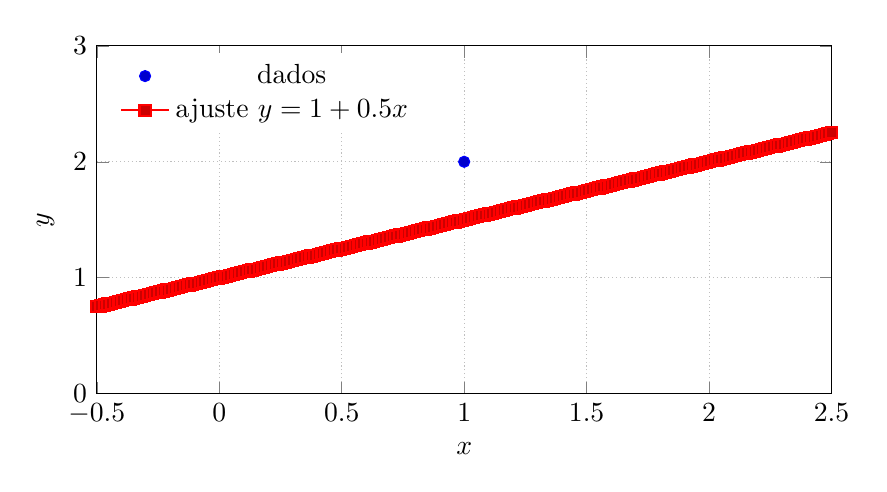
\begin{tikzpicture}
\begin{axis}[
  width=0.9\linewidth, height=6cm,
  xlabel={$x$}, ylabel={$y$},
  xmin=-0.5, xmax=2.5, ymin=0, ymax=3,
  grid=both, grid style={densely dotted},
  legend style={at={(0.02,0.98)},anchor=north west,draw=none}
]
  \addplot+[only marks,mark=*] coordinates {(0,1) (1,2) (2,2)}; \addlegendentry{dados}
  \addplot+[domain=-0.5:2.5, samples=200, thick] {1 + 0.5*x}; \addlegendentry{ajuste $y=1+0.5x$}
\end{axis}
\end{tikzpicture}
\caption{Exemplo de ajuste linear por mínimos quadrados. A reta não passa por todos os pontos, mas minimiza o erro global.}
\label{fig:ls-fit}
\end{figure}

%---------------------------------------------------------
\section{Ligação com assimilação de dados}
O método dos mínimos quadrados é a espinha dorsal da formulação estatística da assimilação de dados.  
Na AD, o funcional a minimizar tem estrutura análoga à de \eqref{eq:J_scalar}, porém com dois termos principais:
\begin{equation}
J(x) = (x - x_b)^\top B^{-1} (x - x_b)
     + (y - Hx)^\top R^{-1} (y - Hx),
\label{eq:J-DA}
\end{equation}
em que o primeiro termo mede o erro do modelo e o segundo, o das observações.  
Minimizar $J$ equivale a resolver uma versão generalizada do problema de mínimos quadrados ponderado por covariâncias — uma generalização direta de \eqref{eq:normal-equations}.

%---------------------------------------------------------
\section{Síntese}
O método dos mínimos quadrados marca a transição entre a interpolação determinística e a assimilação estatística.  
O conceito de \emph{melhor estimativa global} substitui o de \emph{ajuste exato}, preparando o caminho para a \emph{análise objetiva} e, mais adiante, para a formulação completa da assimilação de dados.  
No próximo capítulo, exploraremos como essa ideia se expande para duas dimensões e como a suavização controla o equilíbrio entre fidelidade e coerência espacial.

% Fim do Capítulo 3
